\section{本誌 概要}\label{ux6628ux4ecaux306ediyux4e8bux60c5}

本誌ではロボットハードウェア製作において、モータ回転数制御の実現方法を記載しています。
具体的な題材として、毎年川崎市で開催されている
「かわさきロボット競技大会」の機体製作を取り上げます。

\section{かわさきロボット競技大会の概要}\label{ux672cux8a8cux306eux4e2dux8eab}

かわさきロボット競技大会では、リング上で2台のロボットを戦わせます。
勝敗は審判の判定によって決定されます。
勝利条件の概略は下記の通りです。(大会HP\cite{kawasaki_public_HP}を参照)

\begin{itemize}
\tightlist
\item
  ラウンド内にリングの場外へ相手機体を押し出す
\item
  ラウンド内にリング上で相手機体をダウン(走行不可能な状態)させ、\\
  10カウントダウン状態をキープする
\end{itemize}

製作する機体の概略は下記の通りです。
詳細はかわさきロボット競技大会公式サイト\cite{kawasaki_public_HP}に記載されています。
参考までに筆者が過去に製作した機体はFig.\ref{fig101}です。

\begin{itemize}
\tightlist
\item
  サイズ制限:全幅250mm × 全長350mm × 高さ700mm(スタート時)
\item
  重量制限:3300g以内
\item
  操縦は、競技大会の実行委員会が規定するプロポを用いること
\item
  ロボットには、それぞれ1セット以上の脚機構、アーム機構が搭載されていること
\item
  ロボットは走行用の脚部と相手機体への攻撃用のアーム部を有する
\end{itemize}

\begin{figure}[htbp]
\centering
\includegraphics[width=380pt]{fig/fig101.eps}
\caption{筆者のかわさきロボット出場機体}
\label{fig101}
\end{figure}


\section{ロボット操縦の課題}\label{ux672cux8a8cux306eux5bfeux8c61ux8005}

製作したロボットは例えば左右の脚ユニットの負荷ばらつき、モータの性能ばらつき等で
同じ操作量を入れてもFig.\ref{fig102}のように思った方向に進まない場合があります。

\begin{figure}[htbp]
\centering
\includegraphics[width=280pt]{fig/fig102.eps}
\caption{ロボットの動き}
\label{fig102}
\end{figure}

そこで、Fig.\ref{fig103}のようにモータの回転数に対して
フィードバック制御を入れ、左右の回転数差を無くします。

\begin{figure}[htbp]
\centering
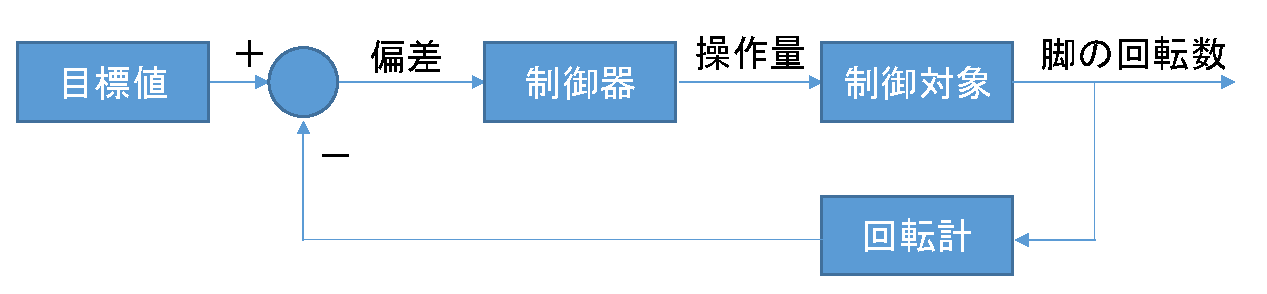
\includegraphics[width=280pt]{fig/fig103.eps}
\caption{フィードバック制御}
\label{fig103}
\end{figure}

ロボット制御システムのハードウェア構成例として、Fig.\ref{fig104}の通りです。
今回、制御プログラムをMatlab/Simulink上で構築してArduinoで動かすことを目指します。

\begin{figure}[htbp]
\centering
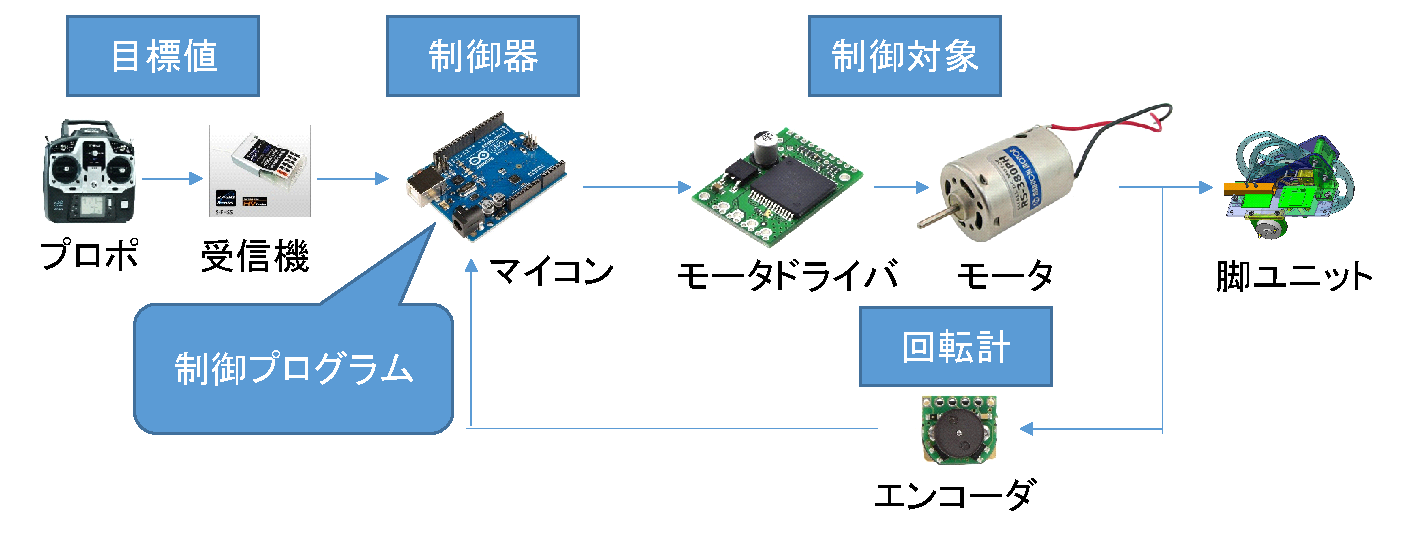
\includegraphics[width=250pt]{fig/fig104.eps}
\caption{ロボット制御システムのハードウェア構成例}
\label{fig104}
\end{figure}


\section{Matlab/Simulink開発環境構築}\label{ux5927ux578bux90e8ux54c1ux306eux4f5cux6210ux65b9ux6cd5}

本書執筆時の動作環境を下記に示します。

\begin{itemize}
  \tightlist
  \item
   OS:Windows 10 64bit
  \item
   Matlab/Simulink:R2018a
   \item
   Arduino:Mega 2560 R3 または Uno R3
\end{itemize}

\subsection{Matlab/Simulinkのインストール}\label{ux6a5fux4f54}

個人ライセンス製品の MATLAB Home \cite{MathWorks_HP} を使います。\\
2018年8月時では、MATLAB本体は¥16,500、Simulinkは¥4,990 です。


\subsection{Simulink での Arduino 動作環境をインストール}\label{ux6a5fux4f55}

Matlab起動時のメニューにある "アドオン" ⇒ "ハードウエアサポートパッケージの入手" を
クリックします。
アドオン エクスプローラーで、
Simulink Support Package for Arduino Hardware (Fig.\ref{fig105}) を
選択してインストールします。

\begin{figure}[htbp]
  \centering
  \includegraphics[width=130pt]{fig/fig105.eps}
  \caption{アドオン エクスプローラー}
  \label{fig105}
  \end{figure}


%\clearpage  
\subsection{C言語コンパイラのインストール}\label{ux5bfeux7b56ux6848}

第3章に記載している S-Function Builder ブロックを使用するためにはC言語コンパイラが必要です。

C言語コンパイラ有無の確認は、Matlab コマンドウインドウに下記を入力して実行します。

mex -setup

C言語コンパイラがすでにインストールされていればFig.\ref{fig107}のような表示が出ます。

C言語コンパイラがインストールされていなければ、インストールが必要です。

今回、C言語コンパイラとして、フリーで入手できる Microsoft Windows SDK 7.1 を使用します。

ただし、Microsoft Windows SDK 7.1 は
最新OSだと通常のやり方ではインストールできません\cite{Win_SDK1} \cite{Win_SDK2}。

Microsoft Windows SDK 7.1 インストール手順のポイントを次に示します。


\subsubsection{i. Visual C++ 2010のランタイムをアンインストールする}\label{sec:section1.4.1-1}

下記プログラムが既にインストールされていると、SDKのインストールに失敗するので\\
"アプリと機能" からアンインストールします。

\begin{itemize}
  \tightlist
  \item
  Microsoft Visual C++ 2010 x86 Redistributable
  \item
  Microsoft Visual C++ 2010 x64 Redistributable
  \end{itemize}


\clearpage
\subsubsection{ii. winsdk-web.exeのインストール}\label{sec:section1.4.1-2}

下記ホームページからインストーラをダウンロードして、インストールします。

\url{http://www.microsoft.com/en-us/download/details.aspx?id=8279}

インストール設定画面において、
Microsoft Visual C++2010 のチェックを外してください (Fig.\ref{fig106}) 。

\begin{figure}[htbp]
  \centering
  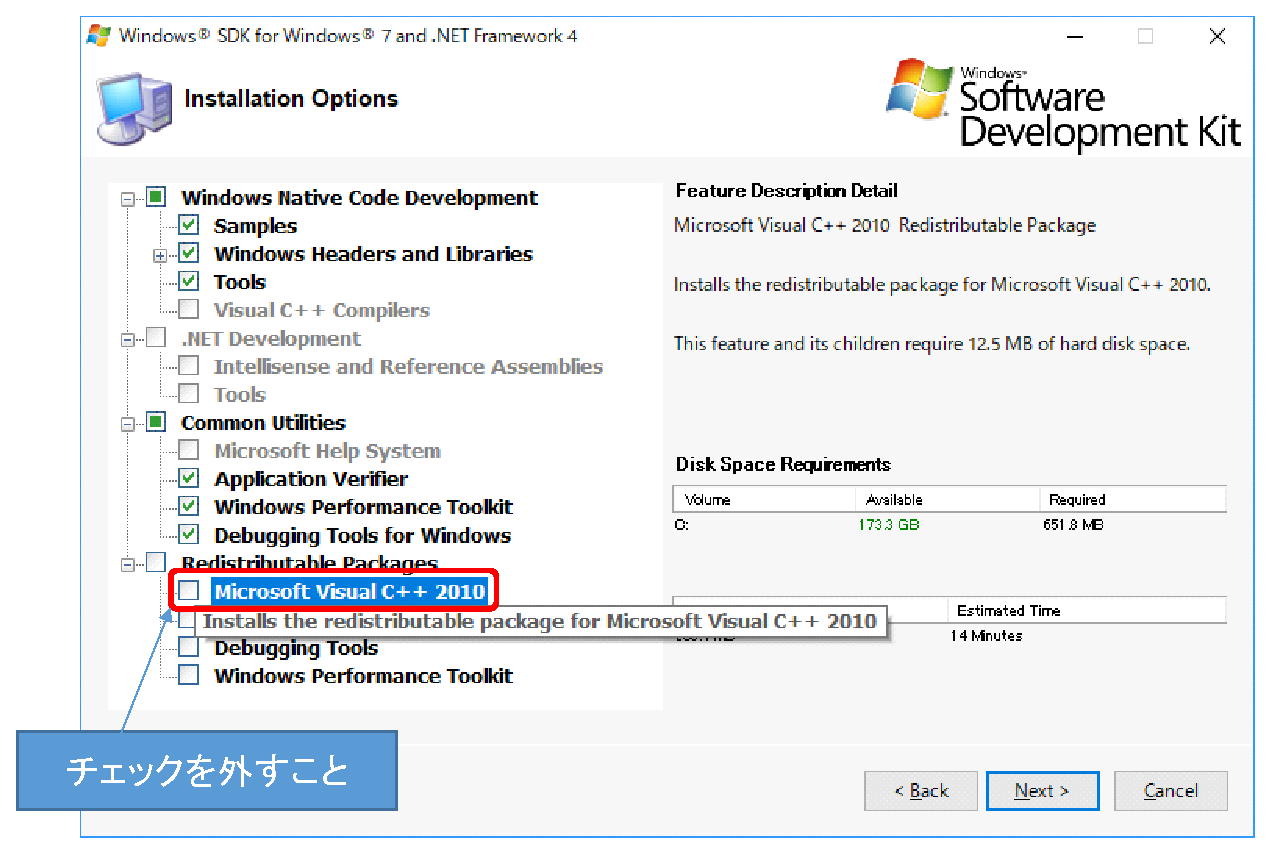
\includegraphics[width=200pt]{fig/fig106.eps}
  \caption{SDK 7.1 インストール設定画面}
  \label{fig106}
  \end{figure}


\subsubsection{iii. VC-Compiler-KB2519277.exeのインストール}\label{sec:section1.4.1-3}

下記ホームページからインストーラをダウンロードして、インストールします。

\url{http://www.microsoft.com/en-us/download/details.aspx?id=4422}

\subsubsection{iv. 正しくインストールされたか確認}\label{sec:section1.4.1-4}

Matlab コマンドウインドウに mex -setup を実行して、
Fig.\ref{fig107}の表示がでればインストールは完了です。

\begin{figure}[htbp]
  \centering
  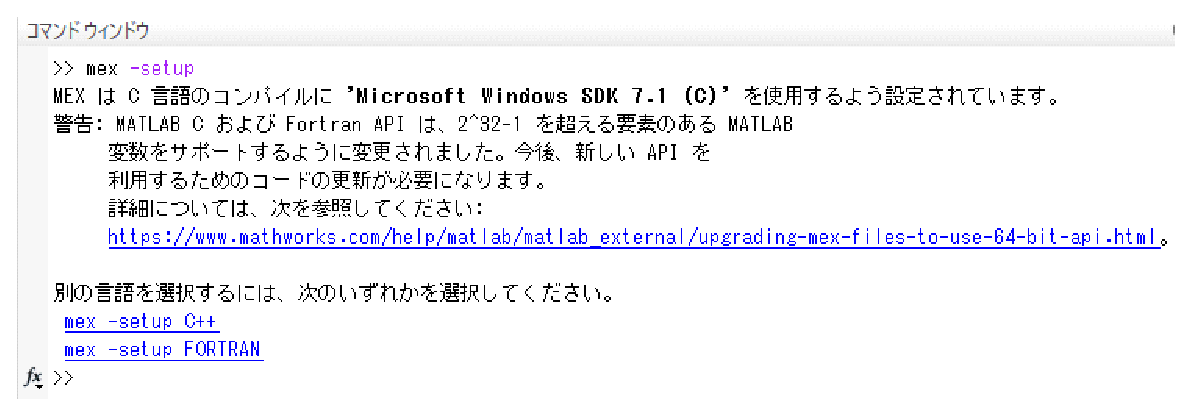
\includegraphics[width=300pt]{fig/fig107.eps}
  \caption{Matlab コマンドウインドウ}
  \label{fig107}
  \end{figure}